\chapter{Application: Identifying Trending Topics on Twitter}
\label{ch:data}

%TODO:
% * Trending now vs trending in window
% * Experimental setup, detection window, etc
% * Minor cleanup (see Devavrat's comments)
% * Plots of data and transformations!!
%   - Show that same transformations applied to different datasets give qualitatively similar results.

In this chapter, we consider the application of the method and algorithm proposed
in chapters \ref{ch:method} and \ref{ch:alg} toward detection of trending topics
on Twitter. we discuss the Twitter service, the collectiion and pre-processing of
data, and the experimental setup for the detection task.

\section{Overview}
\subsection{Overview of Twitter}
Twitter is a real-time messaging service and information network. Users of
Twitter can post short (up to 140 characters) messages called {\em Tweets},
which are then broadcast to the users' {\em followers}. Users can also engage in
conversation with one another. By default, Tweets are public, which means that
anyone can see them and potentially join a conversation on a variety of topics
being discussed. Inevitably, some topics gain relatively sudden popularity on
Twitter. For example, a popular topic might reflect an external event such as a
breaking news story or an internally generated inside joke or game. Twitter
surfaces such topics in the service as a list of Trending Topics. 

\subsection{Twitter-Related Definitions}
Talking about Tweets, topics, trends and trending topics can be ambigious, so
here we make precise our usage of these and related terms.
\begin{itemize}
\item We define a {\em topic} to be a phrase consisting of one or more {\em
  words} delimited by spacing or punctuation. A word may be any sequence of
  characters and need not be an actual dictionary word.
\item A Tweet is {\em about} a topic if it contains the topic as a substring.
\item A {\em trending topic} is a topic that is currently on the list of
  Trending Topics on Twitter. If a topic was ever a trending topic during a
  period of time, we say that the topic {\em trended} during that time period.
\item A trending topic will also occasionally be referred to as a {\em trend}
  for short.
\item The {\em trend onset} is the time that a topic first trended during a
  period of time.
\end{itemize}

\subsection{Problem Statement}
At any given time there are many topics being talked about on Twitter. Of these,
some will trend at some point in the future and others will not. We wish to
predict which topics will trend. The earlier we can predict that a topic will
trend, the better. Ideally, we would like to do this while maintaining a low
rate of error (false detections and false non-detections).

\subsection{Proposed Solution}
Our approach to detecting trending topics is as follows. First, we gather
examples of topics that trended and topics that did not trend during
some period of time. Then, for each topic, we collect Tweets about that topic
and generate a time series of the activity of that topic over time. We then use
those time series as {\em reference signals} (cf. Chapter \ref{ch:method}) and
apply the classification method and algorithm described in Chapters
\ref{ch:method} and \ref{ch:alg}.

\section{Data}
\subsection{Data Collection}
The online time series classification method detailed in Chapters
\ref{ch:method} and \ref{ch:alg} requires a set of reference signals
corresponding to trending topics and a set of reference signals corresponding to
non-trending topics. These reference signals represent historical data against
which we can compare our most recent observations to do classification.

The data collection process can be summarized as follows. First, we collected
500 examples of topics that trended at least once between June 1, 2012 and June
30, 2012 (hereafter refered to as the {\em sample window}) and 500 examples of
topics that never trended during the sample window. We then sampled Tweets from the
sample window and labeled each Tweet according to the topics mentioned
therein. Finally, we constructed a reference signal for each topic based on the
Tweet activity corresponding to that topic.

We obtained all data directly from Twitter via the MIT VI-A thesis
program. However, the type as well as the amount of data we have used is all
publicly available via the Twitter API.

\subsubsection{Topics}
We collected a list of all trending topics on Twitter from June 1, 2012 to June
30, 2012 (the {\em sample window}) as well as the times that they were trending
and their rank in the Trending Topics list on Twitter. Of those, we filtered out
topics whose rank was never better than or equal to 3. In addition, we filtered
out topics that did not trend for long enough (the time of the first appearance
to the time of the last appearance is less than 30 minutes) as well as topics
that reappear multiple times during the sample window (the time of the first
appearance to the time of the last appearance is greater than 24 hours). The
former eliminates many topics that are spurious and only trend for a very short
time. The latter eliminates topics that correspond to multiple events. For
example, the name of a football player might trend every time there is an
important game. We would like to avoid such ambiguity and restrict each trending
topic to correspond to a single underlying event within the sample window.

We collected topics that did not trend during the sample window in two
steps. First, we sampled a list of $n$-grams (phrases consisting of $n$
``words'') occuring on Twitter during the sample window for $n$ up to 5. We
filtered out $n$-grams that contain any topic that trended during the sample
window, using the original, unfiltered list of all topics that trended during
the sample window. For example, if ``Whitney Houston'' trended during the sample
window, then ``Whitney'' would would be filtered out of the list of topics that
did not trend. We also removed $n$-grams shorter than three characters, as most
of these did not appear to be meaningful topics. Lastly, we sampled 500
$n$-grams uniformly from the filtered list of $n$-grams to produce the final
list.

\subsubsection{Tweets}
% TODO: Is 10% accessible publicly? For a price?
We sampled 10\% of all public Tweets from June 1, 2012 to June 30, 2012
inclusive. We labeled each Tweet with the topic or topics contained therein
using a simple regular expression match between the Tweet text and the topic
text. In addition to the Tweet text, we recorded the date and time the Tweet was
authored.

%TODO: Give the parameters names!!!
\subsection{From Tweets to Signals}
We discuss the process of converting the timestamped Tweets for a given topic
into a reference signal. Each of the steps below is followed in order for each
topic.

\subsubsection{Computing Tweet Rate}
First, we determine the rate of Tweets about a topic over time by binning the
Tweets into time bins of a certain length. we used time bins of length two
minutes. 

\subsubsection{Normalizing to Remove Baseline}
A first glance at the data reveals that many non-trending topics have a
relatively high rate and volume of Tweets, and many trending topics have a
relatively low rate and volume of Tweets. One important difference is that many
non-trending topics have a high {\em baseline rate} of activity while most
trending topics are preceded by little, if any, activity prior to gaining sudden
popularity. For example, a non-trending topic such as 'city' is likely to have a
consistent baseline of activity becuase it is a common word. To emphasize the
parts of the rate signal above the baseline and de-emphasize the parts below the
baseline, we divide the rate by the mean rate over the entire window. We then
take the resulting quotient to a power $\beta$, which controls how much we
reward and penalize rates above and below the mean rate. Figure
\ref{fig:spikes_baseline} shows signals without any baseline normalization and
their baseline-normalized versions.

\subsubsection{Rewarding Spikes}
%TODO: This is weak. Do we want to be rewarding big jumps or sudden jumps? Not
%clear which one you're doing here, and not clear which is more justifiable.
Another difference between the rates of Tweets for trending topics and that of
non-trending topics is the number and magnitude of spikes. The Tweet rates for
trending topics typically contains larger and more sudden spikes than that of
non-trending topics. We reward such spikes by emphasizing them, while
de-emphasizing smaller spikes. If the signal so-far in the transformation
process is $r$, we transform it to \[ s(t) = |\dot{r}(t)|^{\alpha},\] or in the
discrete case, \[ s[n] = |r[n] - r[n-1]|^{\alpha},\] where $\alpha > 1$. Figure
\ref{fig:spikes_baseline} shows the effect of this spike-based transformation.

\subsubsection{Slicing}
The signal resulting from the steps so far is as long as the entire time window
from which all Tweets were sampled. Such a long signal is not particularly
useful as a reference signal. Recall from chapter \ref{ch:alg} that to see how
much the recent trajectory of the observed signal resembles part of a reference
signal, we have to traverse the full length of the reference signal in order to
find the piece that most closely resembles the recent observed trajectory. If
the reference signal for topic that trended spans too long of a time window,
only a small portion of it will represent activity surrounding the onset of the
trend. In addition, it is inefficient to compare the recently observed
trajectory to a reference signal that is needleslly long. Hence, it is necessary
to select a small slice of signal from the much longer rate signal. In the case
of topics that trended, we select a slice that terminates at the first onset of
trend. That way, we capture the pattern of activity leading up to the trend
onset, which is crucial for recognizing similar pre-onset activity in the
observed signal. We do not include activity after the true onset because once
the topics is listed in the Trending Topics on Twitter, we expect the
predominant mode of spreading to change. For topics that did not trend, we
assume that the rate signal is largely stationary and select slices with random
start and end times. For simplicity, all slices are a fixed size.

\subsubsection{Smoothing}
Tweet rates, and the aforementioned transformations thereof, tend to be noisy,
especially for small time bins. To mitigate this, we convolve the signal
resulting from the previous step with a smoothing window. Figure
\ref{fig:smooth} shows the effect of smoothing with various window sizes.

\subsubsection{Branching Processes and Logarithmic Scale}
It is reasonable to think of the spread of a topic from person to person as a
branching process. A branching process is a model of the growth of a population
over time, in which each individual of a population in a given generation
produces a random number of individuals in the next generation. While we do not
know the details of how a topic spreads, we do know that in a wide generality of
branching processes, the growth of the population is exponential with time, with
the exponent depending on the details of the model \cite{AthreyaNey} (see
\cite{Szabo} for a treatment involving the spread of topics on Twitter). It is
reasonable, then, to measure the volume of tweets at a logarithmic scale to
reveal these details. Therefore, as a final step, we take the logarithm of the
signal constructed so far. Figure \ref{fig:log} shows a sample of signals and
their log-scaled versions.

\begin{figure}[h!]
\begin{center}
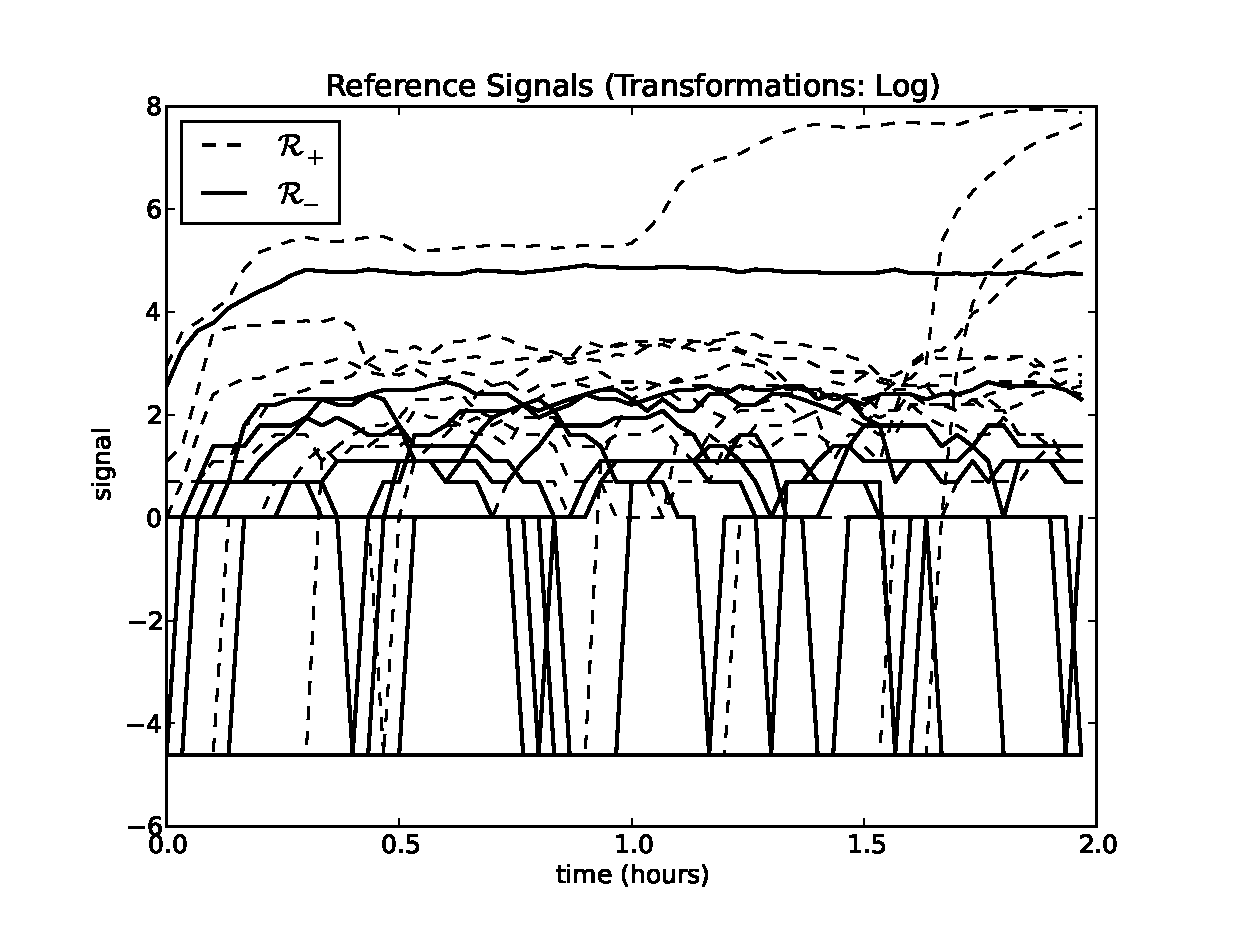
\includegraphics[width=3.10in]{../fig/final/signal_transform/log.eps}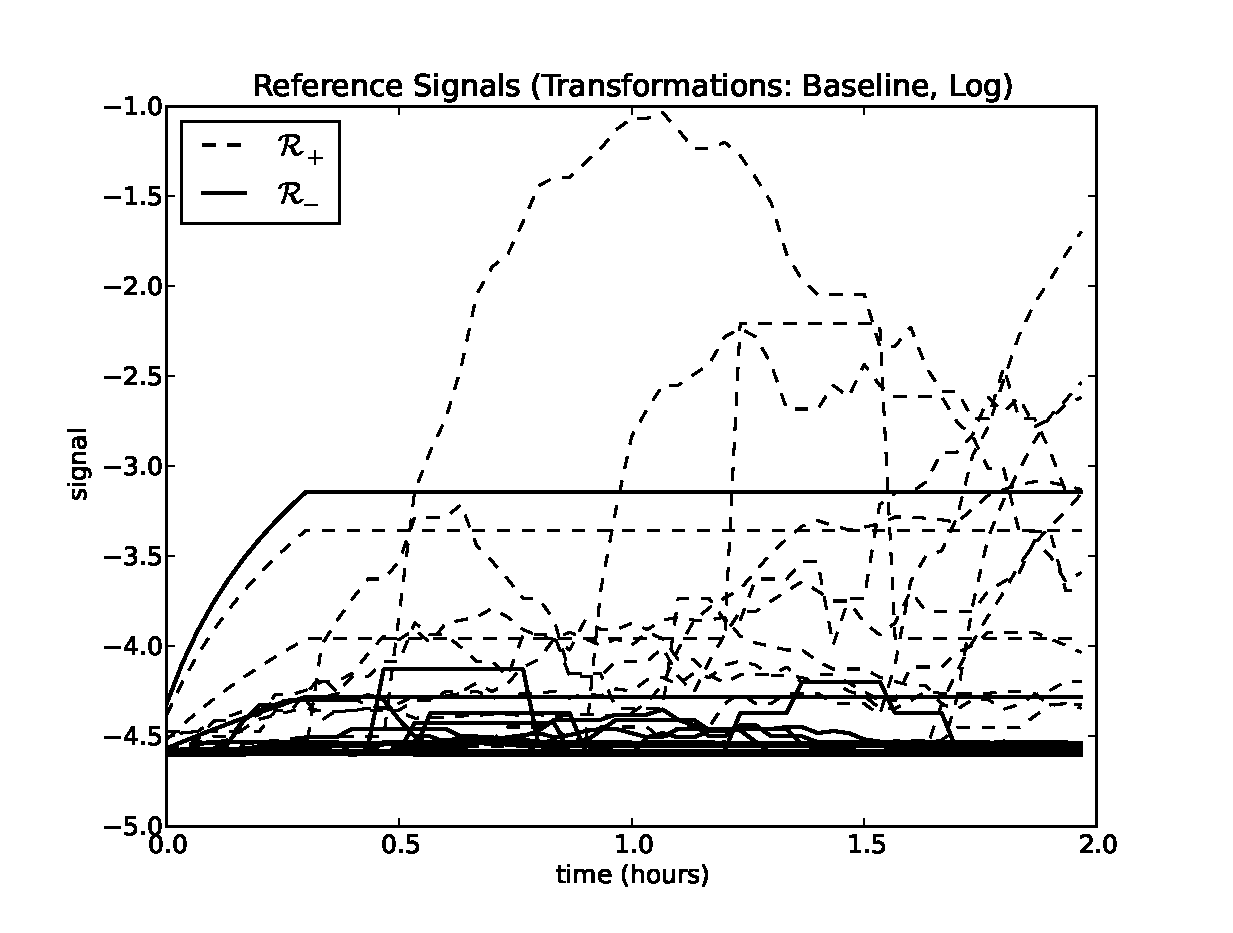
\includegraphics[width=3.10in]{../fig/final/signal_transform/log_baseline.eps}
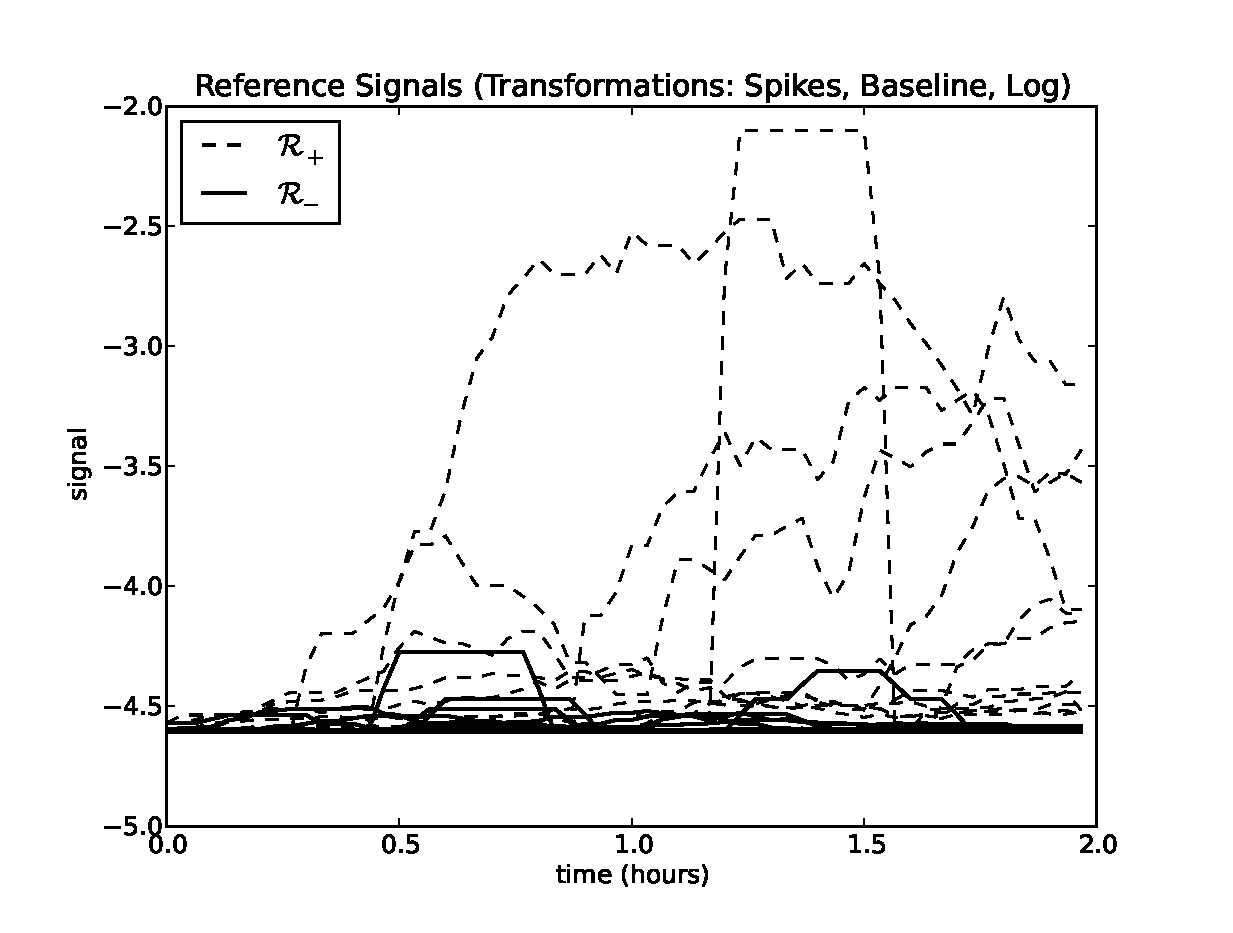
\includegraphics[width=3.10in]{../fig/final/signal_transform/log_baseline_spikes.eps}
\end{center}
\caption{\label{fig:baseline_spikes} Reference signals of either class are hard to tell apart without normalization. {\bf Top left}: no baseline or spike normalization. {\bf Top right}: Baseline normalization. {\bf Bottom}: Baseline and spike-based normalization.}
\end{figure}

\begin{figure}[h!]
\begin{center}
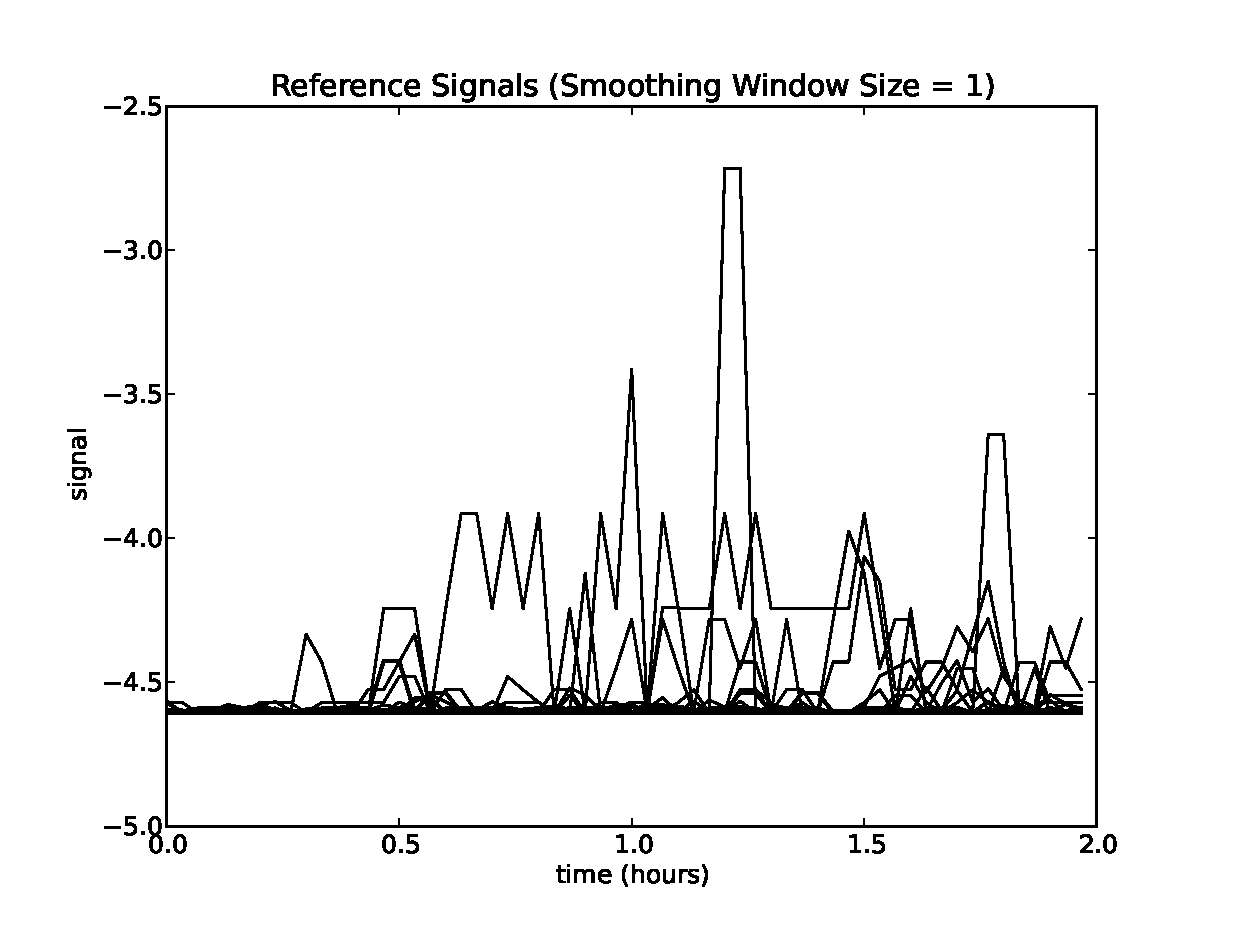
\includegraphics[width=3.10in]{../fig/final/signal_transform/smooth_1.eps}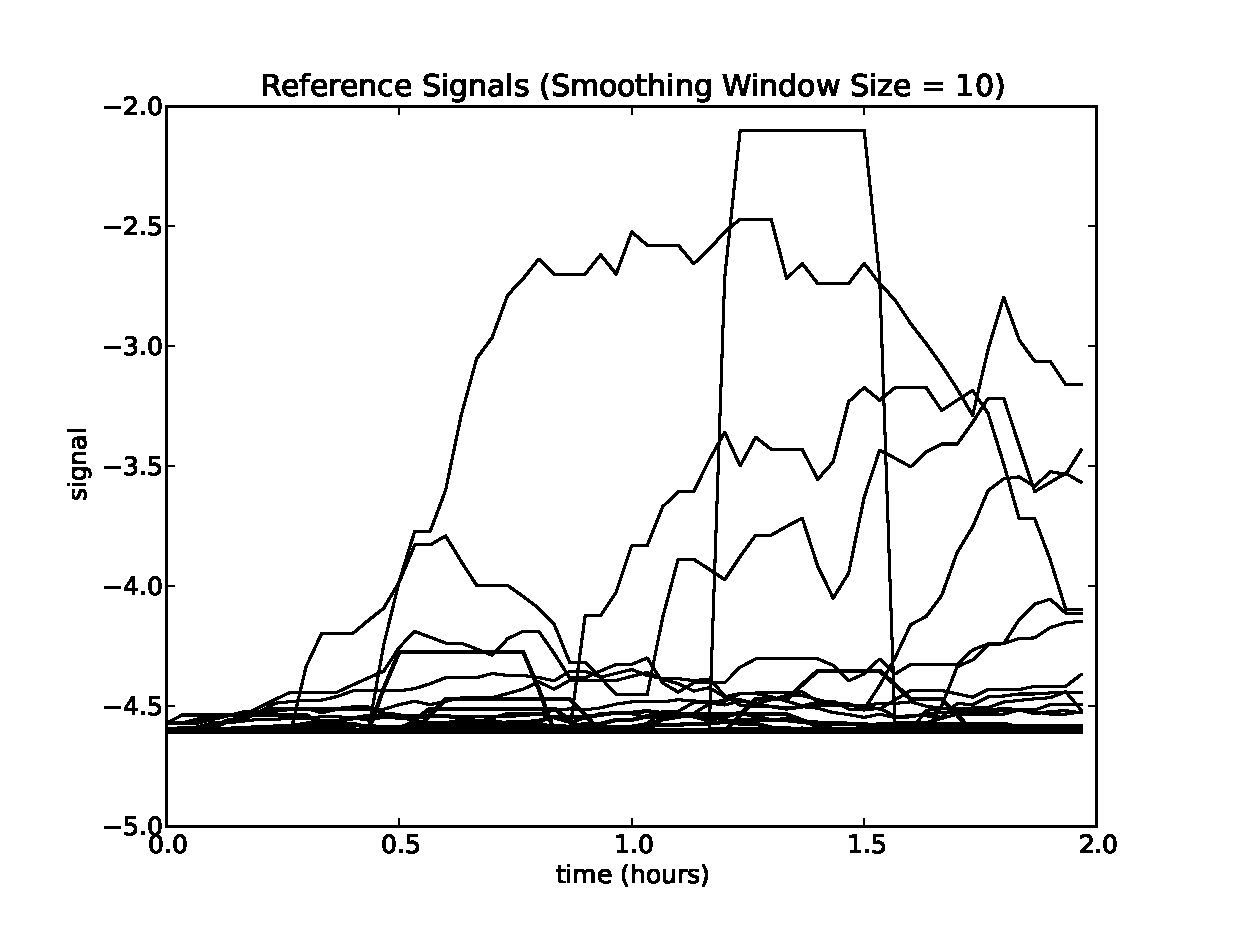
\includegraphics[width=3.10in]{../fig/final/signal_transform/smooth_10.eps}
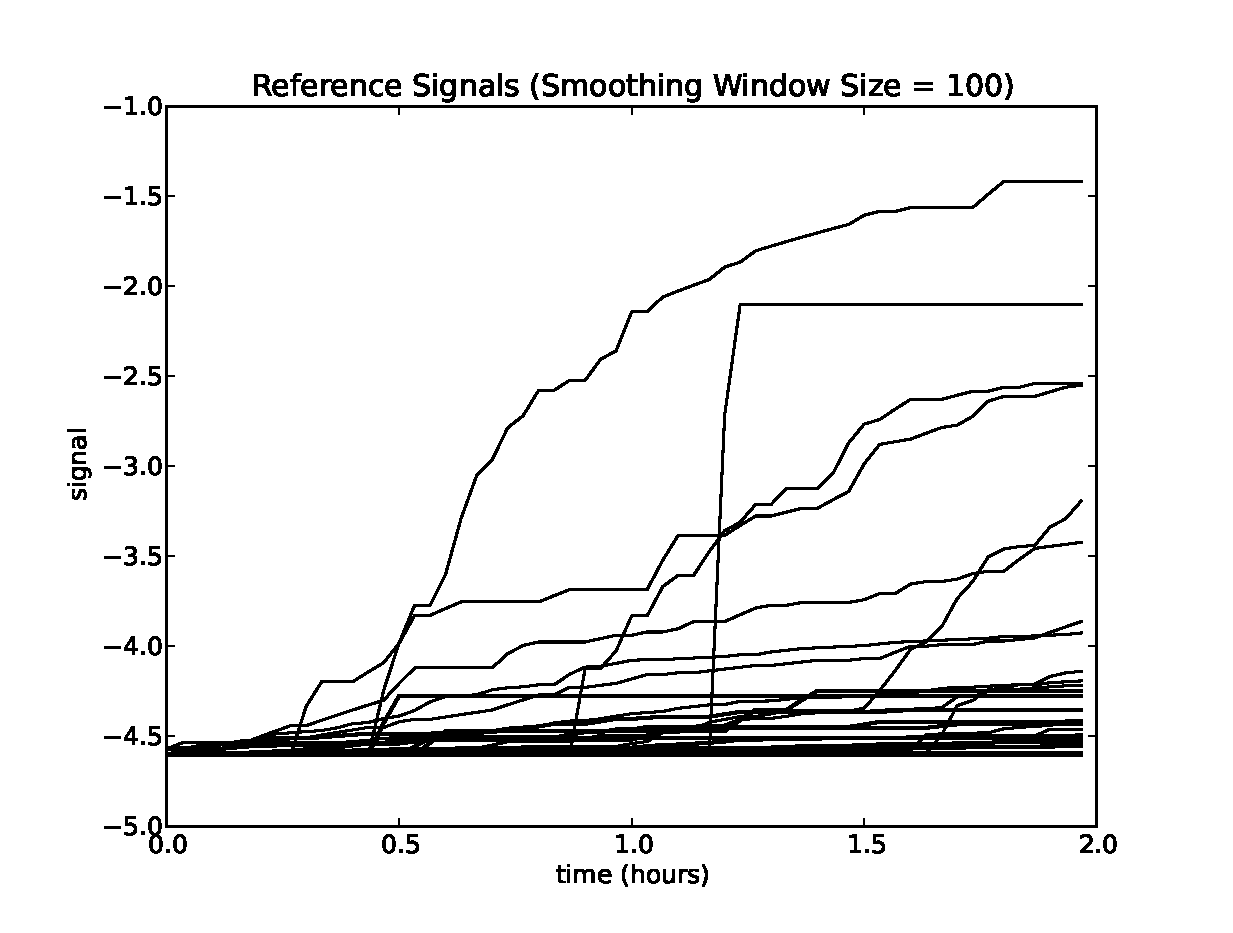
\includegraphics[width=3.10in]{../fig/final/signal_transform/smooth_100.eps}
\end{center}
\caption{\label{fig:smooth} The results of smoothing the reference signals (with spike and baseline normalization previously applied) with windows of size 1 (2 minutes, i.e. no smoothing), 10 (20 minutes), and 100 (3 hours, 20 minutes).}
\end{figure}

\begin{figure}[h!]
\begin{center}
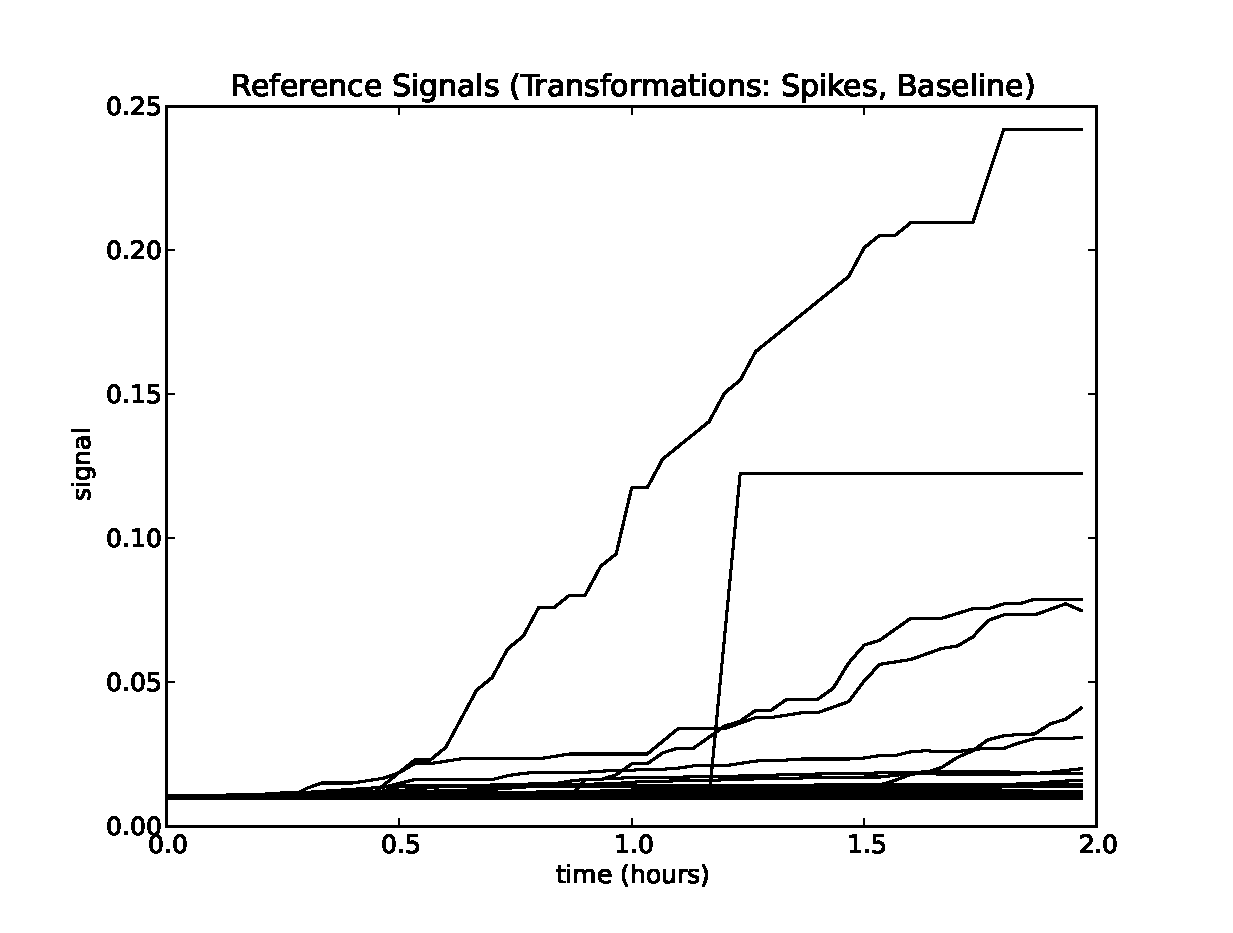
\includegraphics[width=3.10in]{../fig/final/signal_transform/no_log.eps}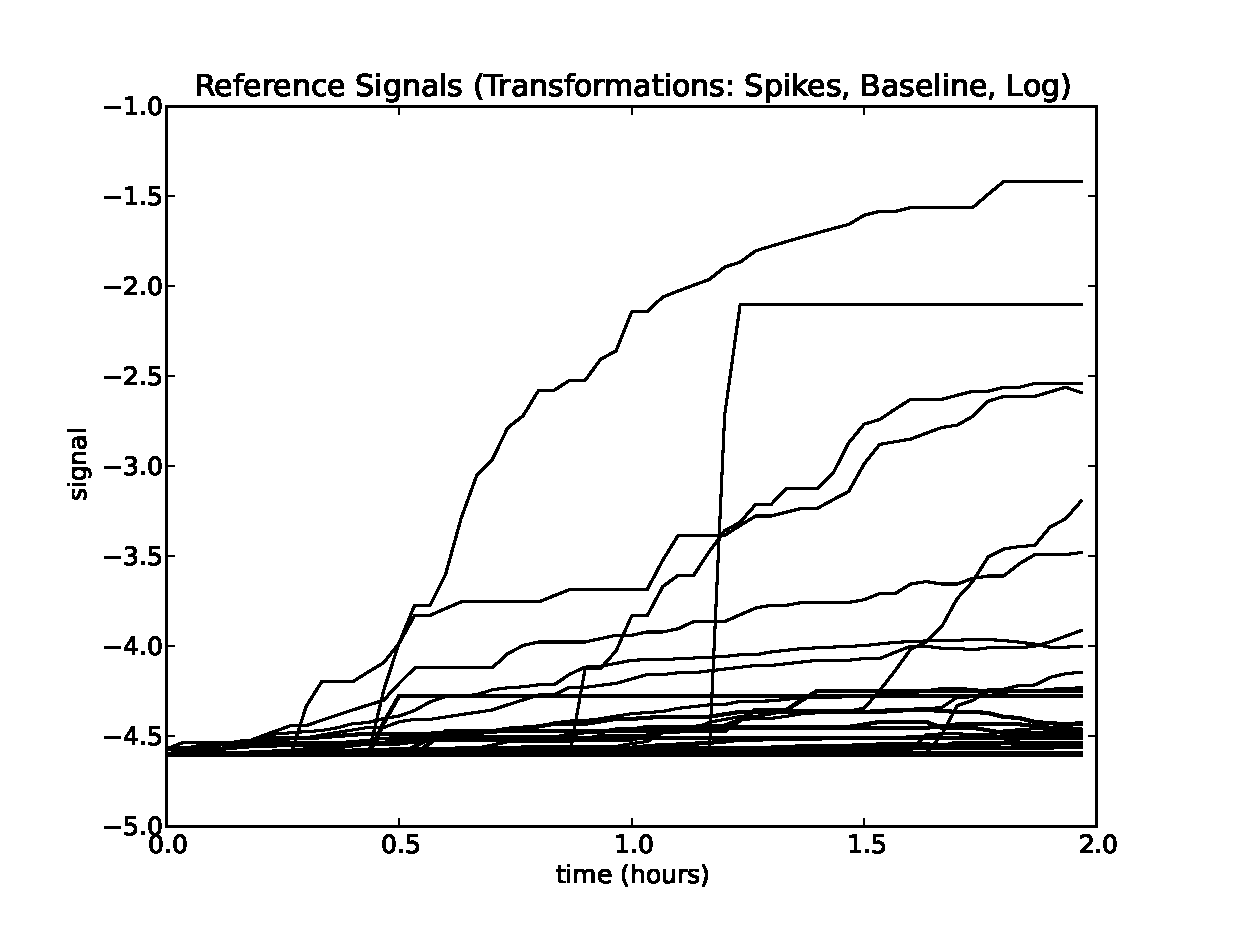
\includegraphics[width=3.1in]{../fig/final/signal_transform/yes_log.eps}
\end{center}
\caption{\label{fig:log} Logarithmically scaled reference signals (with spike and baseline normalization previously applied) allow one to make finer-grained distinctions between signals. {\bf Left}: Not logarithmically scaled. {\bf Right}: Logarithmically scaled.}
\end{figure}

\clearpage

\section{Experiment}
We propose an experiment to measure our algorithm's performance on two fronts:
error rate and relative detection time. We divide the set of topics into a
training set and a test set using a 50/50 split. For each topic in the test
set, we wish to predict if the topic will trend. If the topic really did trend,
we wish to detect it as early as possible relative to the true trend onset while
incurring minimal error.

\subsection{Detection Setup}
In principle, to test the detection algorithm, one would step through the signal
in the entire sample window for each topic in the test set and report the time
of the first detection, or that there were no detections. In practice, we take a
shortcut to avoid looking through the entire signal based on the following
observations about the activity of topics that trended and topics that did
not. First, for topics that trended, there is little, if any activity aside from
that surrounding the true onset of the trend. In the rare event that a detection
is made very far from the true onset, it is reasonable to assume that this
corresponds to a completely different event involving that topic and we can
safely ignore it. Thus, the only part of the signal worth looking at is the
signal within some time window from the true onset of the trend. Second, topics
that did not trend exhibit relatively stationary activity. That is, the signal
usually looks roughly the same over the entire sample window. Therefore, it is
reasonable to perform detection only on a piece of the signal as an
approximation to the true detection performance.

We perform detection over a window of $2N_{obs}$ samples --- twice the length of a
reference signal. For convenience and future use, we define this in terms of hours.

\begin{defn}
Let $h_{ref}$ be the number of hours corresponding to $N_{ref}$ samples. At 2 minutes per sample, $h_{ref}$ is given by $N_{ref} / 30$.
\end{defn}

For test topics that have trended, we do detection on the window spanning
$2h_{ref}$ hours centered at the true trend onset. For topics that did not
trend, we randomly choose a window of the desired size. Note that, although this
seems to require {\em a priori} knowledge of whether the test topic ever trended
or not, this is only a consequence of the shortcut we take to not do detection
over the entire sample window.

\subsection{Parameter Exploration}
